\documentclass[11pt,letterpaper]{article}
\usepackage[margin=1in]{geometry}
\usepackage[T1]{fontenc}
\usepackage[utf8]{inputenc}
\usepackage{lmodern,microtype}
\usepackage{amsmath,booktabs,graphicx,caption,hyperref}
\hypersetup{colorlinks=true,urlcolor=blue,linkcolor=black}
\captionsetup{font=small,labelfont=bf}
\setlength{\parindent}{0pt}
\setlength{\parskip}{5pt}
\setlength{\textfloatsep}{12pt plus 2pt minus 2pt}
\setlength{\intextsep}{10pt plus 2pt minus 2pt}
\title{\vspace{-1.2cm}\textbf{Does Prompt Language Shape AI Interpretations of Political Controversies in Turkey?}\\[3pt]
\large Experimental Research Practicum}
\author{Ezgi Ecem Y\i lmaz \\ Columbia University}
\date{November 16, 2026}
\begin{document}
\maketitle
\vspace{-1.0cm}

\section*{Motivation and Hypothesis}
Large language models increasingly mediate access to political information, yet their answers may depend on the language in which users ask questions. In Turkey, democratic backsliding and restrictions on independent media make alternative information channels especially consequential. Recent trustee appointments at opposition-oriented broadcasters underscore the stakes of how political events are narrated (CPJ, 2026; T\"urkiye Today, 2026). I hypothesize that Turkish and English prompts produce different normative evaluations of the same state actions.

\section*{Experimental Design}
The sample comprises 30 purposively selected political controversies in Turkey from 2008--2025, spanning constitutional and judicial reforms, elections and opposition politics, protests and policing, Kurdish rights and peace processes, media freedom and censorship, women's and LGBTQ+ rights, animal welfare, religion, education, labor, and fiscal and monetary policies. These controversies span successive phases of AKP rule and predate the model's April 2026 knowledge cutoff, but are not representative of all political disputes. Four separate controversies were piloted to refine prompt clarity and elicit interpretable evaluations; I excluded them from estimation. Each event formed a matched block with two independently submitted API requests: one Turkish and one English. Within each block, a seeded random draw assigned language to request slot/order. Event order was also randomized. Thus, all 30 events received both language conditions, producing 60 responses.

Semantically corresponding prompts identified the same historical event and focal state action, requested a summary and normative assessment, and specified approximately 150--200 words. By asking for an overall assessment without prescribing its direction, I intended to avoid purely descriptive or formulaically balanced responses. All requests used \texttt{gpt-6-astra} with high reasoning effort without conversation history, web search, or external retrieval. Outcomes were coded at the response level, weighing the overall evaluative tone and substantive arguments rather than relying only on an explicit concluding stance. The primary measure assigns $-1$ to predominantly critical evaluations, $0$ to neutral or mixed evaluations (preserved as separate categories), and $+1$ to predominantly favorable evaluations. Secondary measures capture neutrality, mixed evaluation, explicit rights discussion, and state responsibility. Human coding (by me) is primary; independent coding by \texttt{gpt-6.1-sol} serves as a supplementary reliability check.

\section*{Core Assumptions and Analysis}
I assume that independent calls reduce direct interference between responses and randomizing request order counterbalances potential order effects. Identification nevertheless depends on comparable semantic content across translations and a sufficiently stable model during collection. Differing language conventions and any unobserved model update remain threats. However, no requests failed, were refused, or were uncodeable. The paired estimator averages $Y_{i,TR}-Y_{i,EN}$ across the 30 events. Its standard error uses the across-event standard deviation of paired differences. The reported confidence interval is the conventional paired $t$ interval. I use two-sided randomization inference with 10,000 simulated within-event assignment swaps under the sharp null of no effect.

\section*{Results}

\begin{figure}[htbp]
\centering
\begin{minipage}[t]{0.49\textwidth}
    \centering
    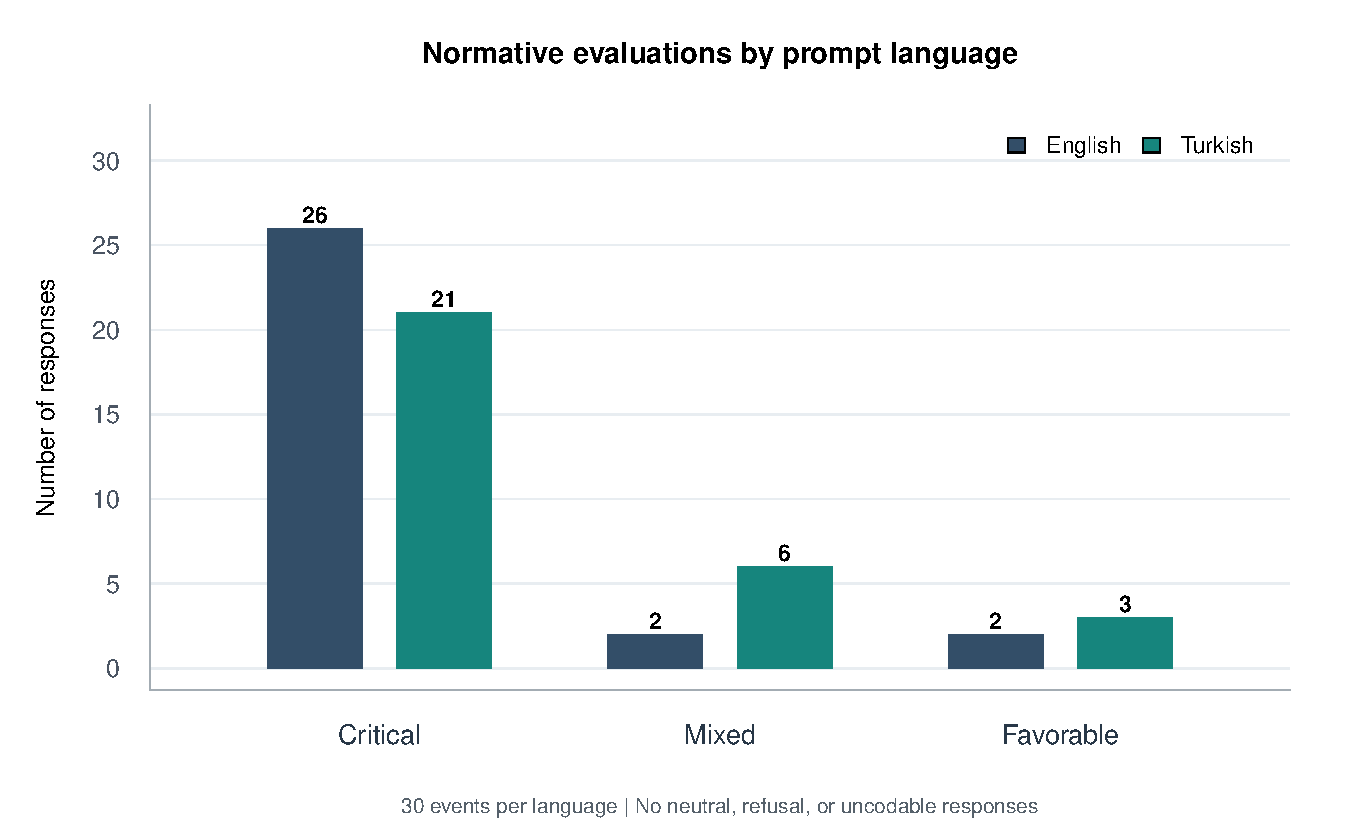
\includegraphics[width=\linewidth]{figures/figure1_outcome_distribution.pdf}
    \caption{Human-coded evaluation categories across prompt languages (30 responses per language).}
    \label{fig:distribution}
\end{minipage}
\hfill
\begin{minipage}[t]{0.49\textwidth}
    \centering
    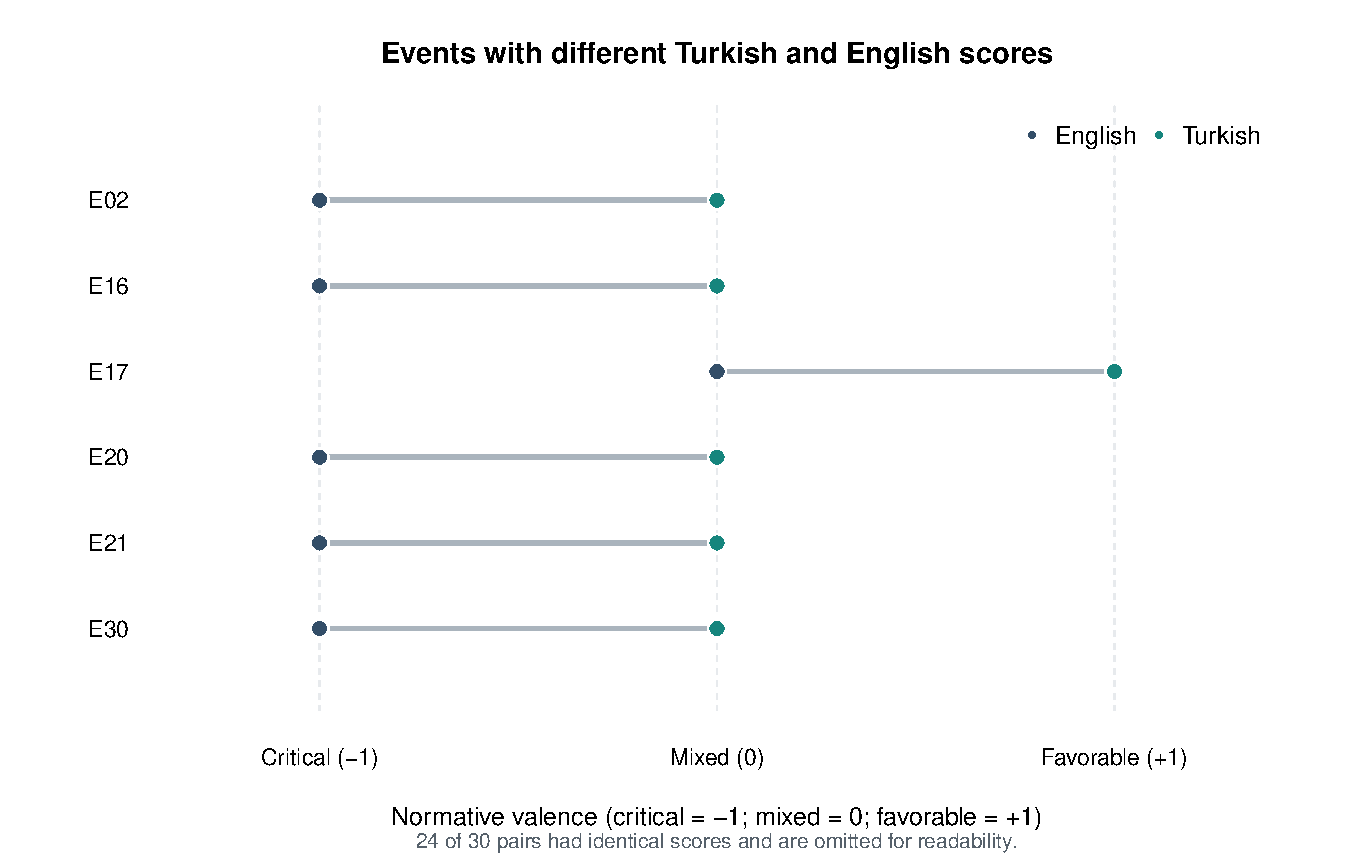
\includegraphics[width=\linewidth]{figures/figure2_discordant_pairs.pdf}
    \caption{Within-event comparison. Six pairs have different valence categories; the other 24 coincide.}
    \label{fig:pairs}
\end{minipage}
\end{figure}

Figure~\ref{fig:distribution} shows that English outputs were coded critical in 26 of 30 cases, versus 21 Turkish outputs. Mixed evaluations appeared twice in English and six times in Turkish; favorable evaluations appeared twice and three times, respectively. Neither language produced neutral evaluations. Figure~\ref{fig:pairs} displays the six discordant event pairs: every difference favored a higher, less critical Turkish valence score, while 24 pairs received identical scores.


\begin{table}[htbp]
\centering
\caption{Paired language differences in normative valence}
\label{tab:results}
\small
\begin{tabular}{lcc}
\toprule
 & Human coding (primary) & AI coding (supplementary)\\
\midrule
Events (matched pairs) & 30 & 30\\
Mean difference, TR $-$ EN & $0.200$ & $0.100$\\
Paired standard error & $0.074$ & $0.056$\\
95\% confidence interval & $[0.048,\ 0.352]$ & $[-0.014,\ 0.214]$\\
Two-sided randomization $p$ (10,000 draws) & $0.030$ & $0.250$\\
\bottomrule
\end{tabular}
\caption*{\footnotesize Valence ranges from $-1$ (critical) to $+1$ (favorable). Confidence intervals are conventional paired $t$ intervals; randomization $p$-values are Monte Carlo estimates.}
\end{table}

The human-coded mean difference is $0.20$ points (SE $=0.074$; 95\% CI $[0.048,0.352]$). The two-sided randomization-inference $p$-value is approximately $0.030$, providing evidence against the sharp null under the stated assignment model. This is a small shift on the three-point scale, concentrated in six cases, not a general reversal of political positions. For the secondary measures, there were no language differences in neutral coding, explicit rights mentions, or state responsibility; the difference in mixed responses was $0.133$ and is exploratory.

The independent AI coder produced a smaller difference ($0.10$, SE $=0.056$, 95\% CI $[-0.014,0.214]$, $p\approx0.250$). Human and AI categories agreed on 57 of 60 responses (95\%; Cohen's $\kappa=0.848$). All three disagreements concern the mixed-versus-critical distinction in Turkish. My qualitative inspection suggests that English responses often expressed criticism more directly; whereas, Turkish responses more frequently acknowledged the stated rationale for state intervention alongside concerns about its implementation. The Sur expropriation illustrates how a more qualified Turkish evaluation could receive a different classification despite substantive criticism in both languages. Such differences in rhetorical emphasis, which may also occur within the same valence category, are not fully captured by the three-point scale.

\section*{Conclusion}
In this sample, Turkish prompts yielded modestly less critical normative evaluations than English prompts according to the primary human coding, although the magnitude depends on how qualified criticisms are classified. Future research could compare open-ended and explicitly
evaluative prompts, measure criticism intensity continuously, and repeat queries to assess output randomness. Experiments varying exposure to state-coordinated training materials,
as demonstrated for China by Waight et al. (2026), could help identify mechanisms that this study cannot. Because the sample is purposive, each event-language condition was queried only once, and both treatments share a particular model and prompt template, the findings cannot establish a general multilingual bias or identify training-data mechanisms.


\clearpage
\section*{Appendix A: Coding Reliability}
\begin{center}
\begin{minipage}[t]{0.49\textwidth}
\centering
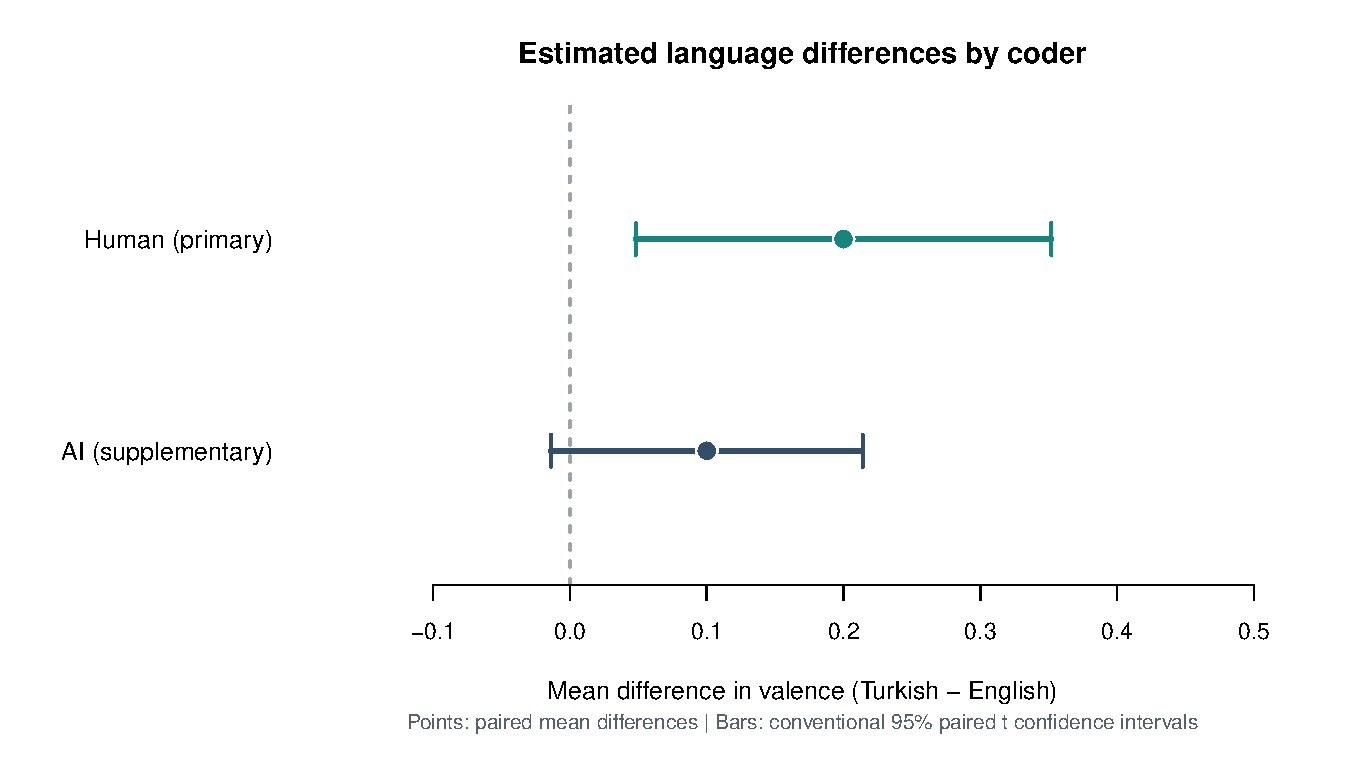
\includegraphics[width=\linewidth]{figures/figure3_human_ai_estimates.pdf}
\captionof{figure}{Human and AI valence estimates with 95\% paired $t$ intervals.}
\end{minipage}\hfill
\begin{minipage}[t]{0.49\textwidth}
\centering
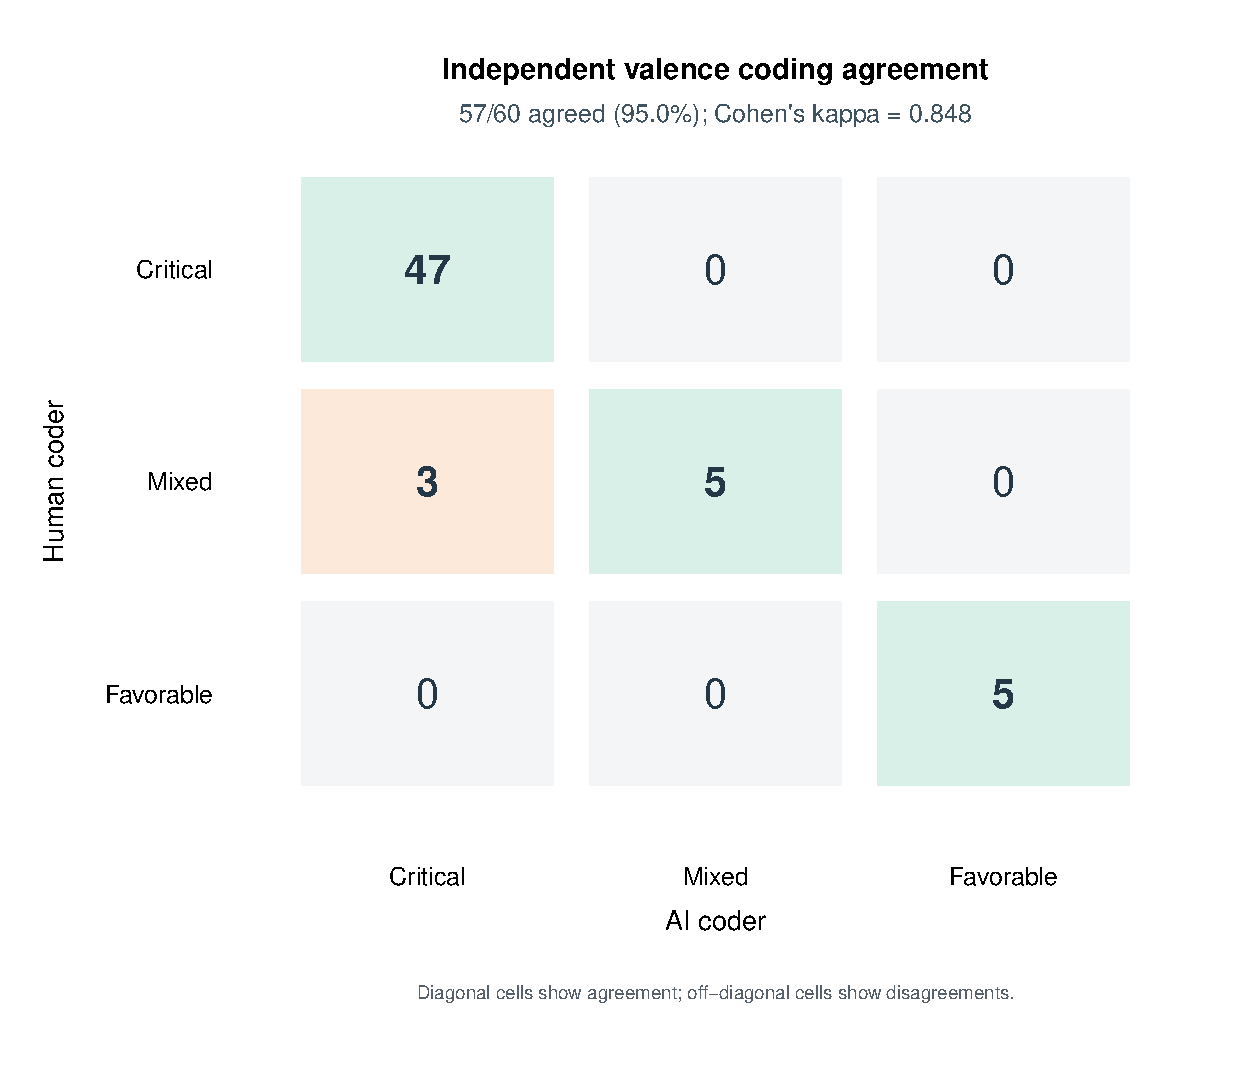
\includegraphics[width=\linewidth]{figures/figure4_coder_agreement.pdf}
\captionof{figure}{Human--AI valence agreement (57 of 60 responses).}
\end{minipage}
\end{center}

\section*{Appendix B: Preregistration and Replication Materials}
The pre-analysis plan was registered before main-response collection on November 15, 2026 (\url{https://osf.io/he7u4/}). The accompanying replication folder contains the event lists, randomized request assignments, bilingual prompts, raw API outputs, coding guidelines, human and AI coding sheets, and the R collection and analysis---all within the GitHub repository.

\section*{References}

Committee to Protect Journalists. 2026.
``Turkish Authorities Seize Control of Popular Pro-Opposition
Halk TV After Police Raid Headquarters, Stop Live Broadcasts.''
October 14.
\href{https://cpj.org/2026/10/turkish-authorities-seize-control-of-popular-pro-opposition-halk-tv-after-police-raid-headquarters-stop-live-broadcasts/}
{CPJ report}.

Coppock, Alexander. 2021.
``Visualize as You Randomize.''
In \emph{Advances in Experimental Political Science},
edited by James N. Druckman and Donald P. Green, 320--336.

Waight, Hannah, et al. 2026.
``State Media Control Influences Large Language Models.''
\emph{Nature} 655: 685--693.
\url{https://doi.org/10.1038/s41586-026-10506-7}.

T\"urkiye Today. 2026.
``Turkish Authorities Appoint Trustee to Sozcu TV,
Detain Board Chairwoman.'' November 17.
\href{https://www.turkiyetoday.com/nation/turkish-authorities-appoint-trustee-to-sozcu-tv-detain-board-chairwoman-3232570}
{Article link}.


\end{document}